\documentclass[12pt,a4paper,utf8]{ctexart}
\usepackage{graphicx}
\usepackage{subfigure}
\usepackage{amsmath}
\usepackage{amssymb}
\usepackage{cases}
\usepackage{subfig}
\usepackage{cite}
\usepackage[ntheorem]{empheq}
\usepackage{enumitem}
\usepackage{fullpage}
\usepackage{cleveref}
\usepackage{cellspace}
\usepackage{listings}
\usepackage{color}
\usepackage{xcolor}      %代码着色宏包
\usepackage{CJK}         %显示中文宏包

\usepackage{setspace}%使用间bai距宏包

\definecolor{gray}{rgb}{0.5,0.5,0.5}
\definecolor{dkgreen}{rgb}{.068,.578,.068}
\definecolor{dkpurple}{rgb}{.320,.064,.680}


% set Matlab styles
\lstset{
   language=Matlab,
   keywords={break,case,catch,continue,else,elseif,end,for,function,
      global,if,otherwise,persistent,return,switch,try,while},
   basicstyle=\ttfamily,
   keywordstyle=\color{blue}\bfseries,
   commentstyle=\color{dkgreen},
   stringstyle=\color{dkpurple},
   backgroundcolor=\color{white},
   tabsize=4,
   showspaces=false,
   showstringspaces=false,
   breaklines,%自动换行
   columns=fixed,
}

\begin{document}
\CJKfamily{zhkai}	


\begin{center}
    \begin{spacing}{2.0}%%行间距变为double-space
        \textbf{\heiti{\zihao {-1} 计算方法  作业三}}
     \end{spacing}
  
  \textbf{姓名 \quad 龚小航 \qquad  学号 \quad PB18151866  \qquad 日期\quad 2020.12.17}
\end{center}
\textit{}
\vspace{\baselineskip}

\begin{enumerate}
\item[第一题] 
  \begin{enumerate}
    \item[$a)$] 任取$1<i,j\leq n, i\neq j$,只需要证明在第一列消去后$a_{ij}^{(1)}=a_{ji}^{(1)}$即可。\\
            第$k$行第一步操作后结果是第一行乘以$-\frac{a_{k1}}{a_{11}}$然后加到第$i$得到的。
            又由于矩阵$A$是对称矩阵,因此$a_{mn}=a_{nm}$。综上,有:
        \begin{eqnarray} 
            a_{ij}^{(1)}&=&a_{ij}-\frac{a_{i1}}{a_{11}}a_{1j}\\
            a_{ji}^{(1)}&=&a_{ji}-\frac{a_{j1}}{a_{11}}a_{1i}\\
                        &=&a_{ij}-\frac{a_{1j}}{a_{11}}a_{i1}\\
                        &=&a_{ij}^{(1)}
        \end{eqnarray}     
            此即需要证明的结论,得出$A^{(1)}$是对称矩阵。

    \item[$b)$] LU分解在本质上是高斯消元法的一种表达形式。实质上是将A通过初等行变换变成一个上三角矩阵,其
            变换矩阵就是一个单位下三角矩阵。利用对称性,构造以下伪代码:\\
            \begin{figure}[h]
                \centering
                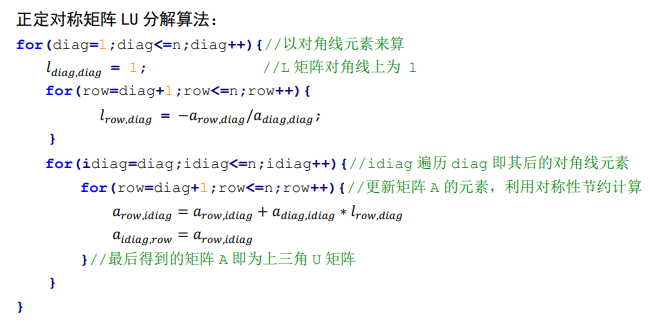
\includegraphics[width=0.9\textwidth]{H3T1B.png}
                \caption{构造正定矩阵LU分解的算法}
            \end{figure}

        
    \item[$c)$] MATLAB程序如下:
    \begin{lstlisting}[frame=single]
format rat
A=[4,-2,4,2;
   -2,10,-2,-7;
   4,-2,8,4;
   2,-7,4,7];
b=[8;2;16;6];
l=zeros(4,4);
n = 4;

%STEP1:求分解出的下三角矩阵L
for j = 1 : n
    sum2=0;
    for k=1:j-1
        sum2 = sum2+l(j,k)*l(j,k);   
    end
    l(j,j) = sqrt(A(j,j)-sum2);
    for i = j+1 : n
        sum=0;
        for k=1:j-1
            sum  = sum+l(j,k)*l(i,k);   
        end
        l(i,j) = (A(i,j)-sum)/l(j,j);
    end
end

l
l*l'

%STEP2:求解下三角方程组Ly=b得y
y = zeros(n,1);
y(1)=b(1)/l(1,1);
for i = 2 : n
    sum = 0;
    for k = 1 : i-1
        sum = sum + l(i,k)*y(k); 
    end
    y(i) = (b(i)-sum)/l(i,i)
end

%STEP3:求解上三角方程组L^T x = y得x
x = zeros(n,1);
x(n) = y(n)/l(n,n);
for i = n-1 : -1 : 1
    sum = 0;
    for k = 1 : n
        sum = sum + l(k,i)*x(k);
    end
    x(i)=(y(i)-sum)/l(i,i);
end
x

    \end{lstlisting}
        运行结果如图所示。从图中可知分解出的下三角矩阵L以及解出的x。\\
        \begin{figure}[h]
            \centering
            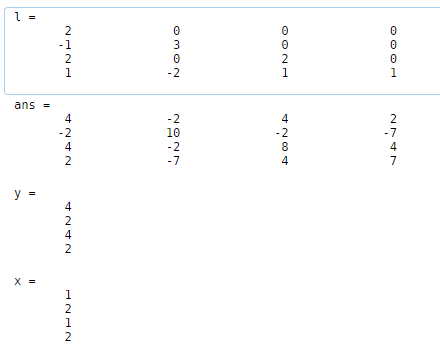
\includegraphics[width=0.6\textwidth]{H3T1C.png}
            \caption{上述程序运行结果}
        \end{figure}
  \end{enumerate}
\item[第二题]
  \begin{enumerate}
    \item[$a)$] 先将迭代格式展开,将迭代矩阵表示出来:
        \begin{eqnarray} 
            x^{(k+1)} &=& (\frac{I}{\omega})^{-1}(\frac{I}{\omega}-A)x^{(k)}+(\frac{I}{\omega})^{-1}b\\
                      &=& \omega I(\frac{I}{\omega}-A)x^{(k)}+\omega Ib\\
                      &=& (I-\omega A)x^{(k)}+\omega b
        \end{eqnarray} 
            由于矩阵$A$是正定矩阵,因此若$A$的特征值记作$\lambda_{1},\lambda_{2},···,\lambda_{n}$
            时,必有$\lambda_{i}>0, 0\leq i\leq n$;题中已经给出了$A$的最小/最大特征值为$\lambda_{1},\lambda_{n}$,
            迭代矩阵的特征值为$1-\omega \lambda_{i}$。\\
            迭代收敛的充分必要条件是迭代矩阵的谱半径小于$1$,由于$\lambda_{i}>0$,只需要让迭代矩阵的特征值不小于$-1$即可。
            而$\omega < 2/\lambda_{n}$时,$1-\omega \lambda_{i}>-1$因此当$\omega$满足题中给出的条件时迭代矩阵的谱半径
            必然小于$1$。即迭代方法收敛。
    \item[$b)$] 对一个对称矩阵$T$,收敛速度$R(T)=-ln \rho (T)$,因此想要收敛速度最快只需要令这个矩阵的谱半径尽量小即可。
            而谱半径是矩阵绝对值最大的特征值。因此$\omega$的最佳值满足使 $max{|1-\omega \lambda_{i}|,1\leq i\leq n}$ 最小。
            由题意可知$\omega>0$,而$A$为正定矩阵,$\lambda_{i}>0$。因此$\rho(I-\omega A)$随$\lambda$增大单调递减,随$\omega$
            增大也单调递减。记$F()$为矩阵的特征值,则有:
        \begin{eqnarray} 
            1-\omega \lambda_{n} \leq F(I-\omega A) \leq 1-\omega \lambda_{1}
        \end{eqnarray}
            而另一方面,$\omega$变化时最好的结果就是令$\rho(I-\omega A)$的上限尽可能小,下限尽可能大。也就是说它们互为相反数,此时
            若$\omega$稍大一点则下限负的更多,稍小一点则上限正的更多:
        \begin{eqnarray} 
                1-\omega_{b} \lambda_{n} + 1-\omega_{b} \lambda_{1} &=& 0\\
                \implies \omega_{b} &=& \frac{2}{\lambda_{1}+\lambda_{n}}
        \end{eqnarray}
            接下来计算迭代矩阵$G_{\omega}=I-\omega A$的谱半径。由刚才得出的结论,若$\omega$稍小则上限较大,最大特征值对应
            $1-\omega \lambda_{1}$;若$\omega$稍大,则下限绝对值更大,此时对应$1-\omega \lambda_{n}$,但在算谱半径时需要取
            绝对值;若$\omega$取最佳值时谱半径对应$1-\omega \lambda_{n}=1-\frac{2}{\lambda_{1}+\lambda_{n}} \lambda_{n}=\frac{\lambda_{n}-\lambda_{1}}{\lambda_{n}+\lambda_{1}}$。
            综上:
        \begin{eqnarray} 
            \label{eq6}
            \rho(G_{\omega})=\left\{
            \begin{aligned}
                1-\omega \lambda_{1}                                    & , & \omega \leq \omega_{b} \\
                \frac{\lambda_{n}-\lambda_{1}}{\lambda_{n}+\lambda_{1}} & , & \omega=\omega_{b}\\
                \omega \lambda_{n}-1                                    & , & \omega \geq \omega_{b}.
            \end{aligned}
            \right.
        \end{eqnarray}
    \item[$c)$] 程序如下所示:
        \begin{lstlisting}[frame=single]
%生成正定对称方阵,特征值1,2,3,4,5
M=[1,0,0,0,0;
   0,2,0,0,0;
   0,0,3,0,0;
   0,0,0,4,0;
   0,0,0,0,5];

B=rand(5,5);
[Q,R]=qr(B);%利用Q矩阵得到正交阵

A = Q*M*Q' %同时作相合、相似变换
[x,y]=eig(A);%A即所需随机方阵
y
b = rand(5,1)

format long
x0=[0 0 0 0 0]';
%输出w=0.3情况下的迭代解以及迭代次数
[x,n]=richason(A,b,x0,10e-10,1000)

%以下求w和谱半径之间的关系
T = [1,2,3,4,5]';
w = 0:0.002:0.4; %w<2/5时收敛
p = max(abs(1.-w.*T))

plot(w, p, '-*');
xlabel('w');
ylabel('p(I-wA)');

function [x,n]=richason(A,b,x0,eps,M)
%Richardson法求解线性方程组 Ax=b
%方程组系数矩阵:A
%方程组之常数向量:b
%迭代初始向量:X0
%e解的精度控制:eps
%迭代步数控制:M
%返回值线性方程组的解:x
%返回值迭代步数:n

I =eye(size(A));
x1=x0;
x=(I-0.3*A)*x0+0.3*b;
n=1;

while(norm(x-x1)>eps)
    x1=x;
    x=(I-0.3*A)*x1+0.3*b;
    n = n + 1;
   if(n>=M)
       disp('Warning: 迭代次数太多,现在退出!');
       return;
   end
end

end
        \end{lstlisting}
            运行结果如下图所示:\\
            \begin{figure}[h]
                \centering
                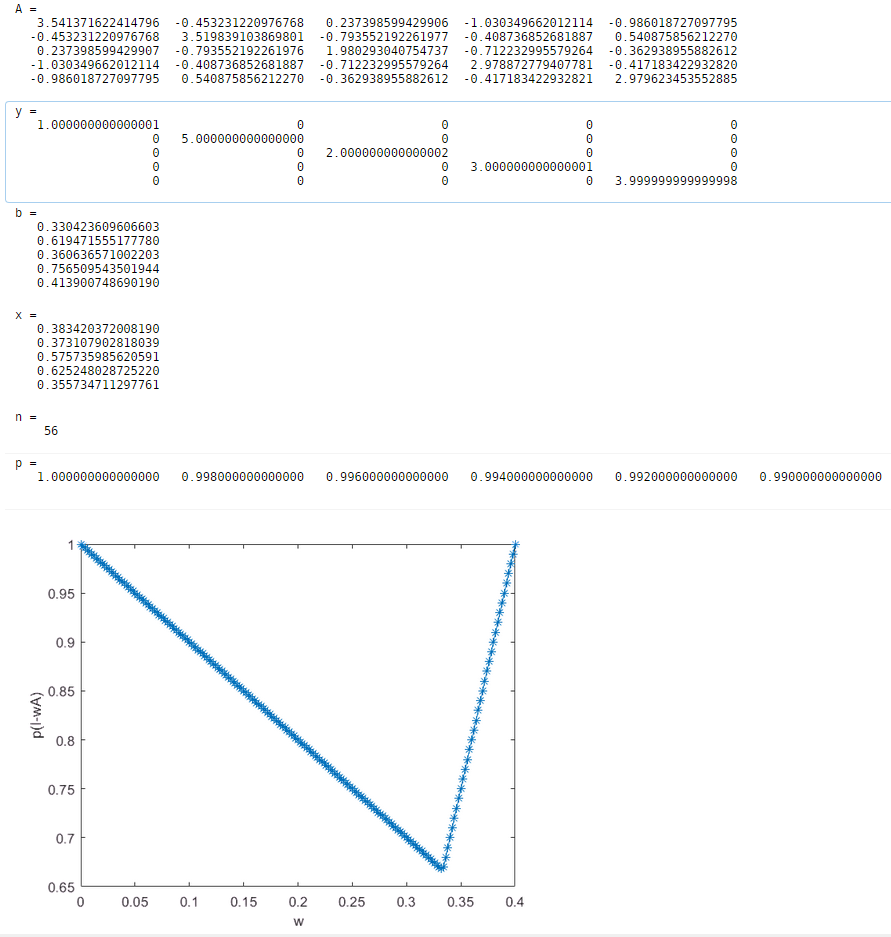
\includegraphics[width=0.9\textwidth]{H3T2C.png}
                \caption{上述程序运行结果图}
            \end{figure}\\
            \\
            \\
            \\
            \\
            可见随机构建的矩阵为A,方程的迭代解为x。最后迭代矩阵的谱半径随$\omega$变化的情况如
            图所示,显然通过对几个点的采样就可以得出$(1)$的结论。

  \end{enumerate}


\item[第三题]
      \begin{enumerate}
        \item[$a)$] 高斯积分$n=6$时,对于任意一个不高于$2n-1$阶的多项式$f(x)$都有:
            \begin{eqnarray} 
                \int_{-1}^{1}f(x)\mathrm{d}x=\sum_{i=1}^{6}\alpha_{i}f(x_{i})
            \end{eqnarray}
            因此就可以得到12个方程组成的非线性方程组:
            \begin{eqnarray} 
                \int_{-1}^{1}x^{k}\mathrm{d}x=\sum_{i=1}^{6}\alpha_{i}x_{i}^{k}, \quad  0\leq k\leq 11
            \end{eqnarray}
            而其中$x_{i},x_{7-i}$关于原点对称,可以简化一部分方程。例如奇次方程积分结果为0。而高斯积分的积分节点和
            积分权重关于原点对称,因此只需要计算6个未知量即可。此处取正半轴的三个节点及其权重。\\
            因此所需方程组为:
            \begin{eqnarray} 
                \int_{-1}^{1}x^{k}\mathrm{d}x=2\sum_{i=1}^{3}\alpha_{i}x_{i}^{k}, \quad   k=0,2,4,6,8,10
            \end{eqnarray}
            总共六个方程。
        \item[$b)$] 写出其雅可比行列式:
            \begin{figure}[h]
                 \centering
                 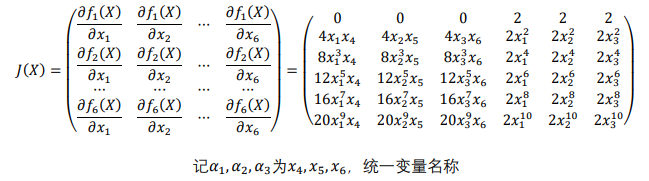
\includegraphics[width=0.9\textwidth]{H3T3B.png}
                 \caption{上述方程组的雅可比行列式}
            \end{figure}
        \item[$c)$] 在$(-1,1)$上等距选取六个积分节点即$-1,-0.6,-0.2,0.2,0.6,1$,在正半轴上即$0.2,0.6,1$。初始的积分权重
                取为$\alpha_{1}=1,\alpha_{2}=1,\alpha_{3}=1$,即等权值即可.\\
                MATLAB程序如下:
            \begin{lstlisting}[frame=single]
x0=[0.2 0.6 1 1 1 1];
[allx,ally,r,n]=mulNewton(fun,x0,1e-8)
%allx用于记录每一步迭代输入的点的矩阵,ally是每一步迭代利用迭代点算得的函数值
function [allx,ally,r,n]=mulNewton(F,x0,eps)
  if nargin==2
    eps=1.0e-8;
  end
  x0 = transpose(x0);
  Fx = subs(F,transpose(symvar(F)),x0);
  var = transpose(symvar(F));
  dF = jacobian(F,var);
  dFx = subs(dF,transpose(symvar(F)),x0);
  n=dFx;
  r=x0-inv(dFx)*Fx';
  n=1;
  tol=1;
  N=100;
  symx=length(x0);
  ally=zeros(symx,N);
  allx=zeros(symx,N);

  while tol>eps
    x0=r;
    Fx = subs(F,transpose(symvar(F)),x0);
    dFx = subs(dF,transpose(symvar(F)),x0);
    r=vpa(x0-inv(dFx)*Fx');
    tol=norm(r-x0)
    if(n>N)
        disp('迭代步数太多,可能不收敛!');
        break;
    end
    allx(:,n)=x0;
    ally(:,n)=Fx;
    n=n+1;
  end
end

function f = fun(x)
  k=6; %1~3为xi,4~6为ai
    for i=1:k
      x(i)=sym (['x',num2str(i)]);
    end 
  f(1)=2*x(4)+2*x(5)+2*x(6)-2;
  f(2)=2*x(4)*(x(1))^2+2*x(5)*(x(2))^2+2*x(6)*(x(3))^2-2/3;
  f(3)=2*x(4)*(x(1))^4+2*x(5)*(x(2))^4+2*x(6)*(x(3))^4-2/5;
  f(4)=2*x(4)*(x(1))^6+2*x(5)*(x(2))^6+2*x(6)*(x(3))^6-2/7;
  f(5)=2*x(4)*(x(1))^8+2*x(5)*(x(2))^8+2*x(6)*(x(3))^8-2/9;
  f(6)=2*x(4)*(x(1))^10+2*x(5)*(x(2))^10+2*x(6)*(x(3))^10-2/11;
end
            \end{lstlisting}
                程序运行结果如下所示:
                \begin{figure}[h]
                    \centering
                    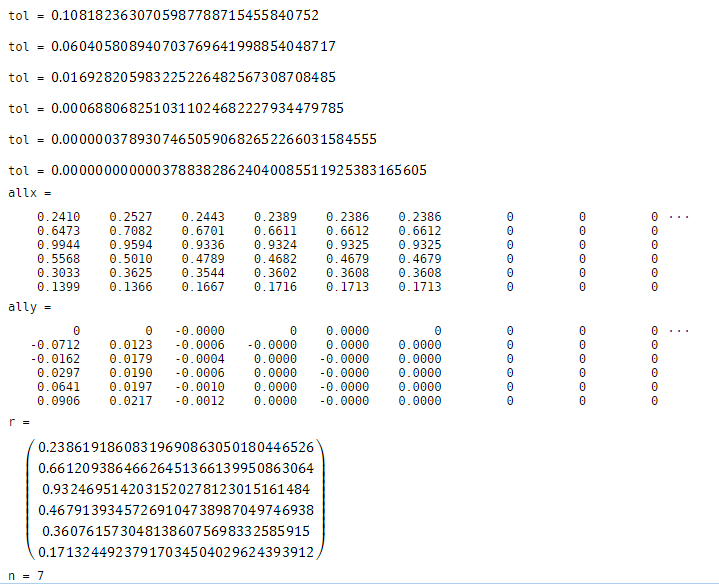
\includegraphics[width=0.9\textwidth]{H3T3C.png}
                    \caption{上述程序运行结果}
               \end{figure}\\
               从图中可知,最后得出的r即为六个未知数的解。即:
            \begin{eqnarray} 
                x=\pm 0.238619186,\quad \alpha=0.467913935\\
                x=\pm 0.661209386,\quad \alpha=0.360761573\\
                x=\pm 0.932469514,\quad \alpha=0.171324492
            \end{eqnarray}
        \item[$d)$] 若在$(-1,1)$上选取切比雪夫点,则选取$n$个点时$x_{i}=cos(\frac{i\pi}{n})$。
                对不同的$n$来说,仍然可以列出$2n-1$个含有$2n-1$个未知数的非线性方程组
            \begin{lstlisting}[frame=single]
for n=2:2:20;
    [x,w]=gauss(n)
    x0=zeros(1,n);
    for i=1:n/2
        x0(i)=cos(i*pi/n);
    end
    for i=n/2+1:n
        x0(i)=cos(i*pi/n);
    end
    [allx,ally,r,n]=mulNewton(fun(n),x0,1e-8)
    
end

function [allx,ally,r,n]=mulNewton(F,x0,eps)
  if nargin==2
    eps=1.0e-8;
  end
  x0 = transpose(x0);
  Fx = subs(F,transpose(symvar(F)),x0);
  var = transpose(symvar(F));
  dF = jacobian(F,var);
  dFx = subs(dF,transpose(symvar(F)),x0);
  n=dFx;
  r=x0-inv(dFx)*Fx';
  n=1;
  tol=1;
  N=100;
  symx=length(x0);
  ally=zeros(symx,N);
  allx=zeros(symx,N);

  while tol>eps
    x0=r;
    Fx = subs(F,transpose(symvar(F)),x0);
    dFx = subs(dF,transpose(symvar(F)),x0);
    r=vpa(x0-inv(dFx)*Fx');
    tol=norm(r-x0)
    if(n>N)
        disp('迭代步数太多,可能不收敛!');
        break;
    end
    allx(:,n)=x0;
    ally(:,n)=Fx;
    n=n+1;
  end
end

function f = fun(n,x)
  k=n;
    for i=1:k
      x(i)=sym (['x',num2str(i)]);
    end 
    for i=1:k
      sum=0;
      for j=1:k/2
         sum=sum+2*x(k/2+j)*x(j)^(2*i-2); 
      end
      f(i)=sum-2/(2*i-1);
    end
end

function [x,w] = gauss(N)
  beta = .5./sqrt(1-(2*(1:N-1)).^(-2));
  T = diag(beta,1) + diag(beta,-1);
  [V,D] = eig(T);
  x = diag(D); [x,i] = sort(x);
  w = 2*V(1,i).^2;
end
            \end{lstlisting}
                对于计算方法来说,只需要将c问的程序函数定义改为由输入n自动生成,然后对不同的
                $n$反复调用即可。迭代算法在n=8时报错,n=6时得出准确解.再计算n=7时的结果,发现
                可以正常运行。因此n最大只能为7
                对比运行结果,在精度$10^{-8}$下程序得到了准确解。
                \begin{figure}[h]
                    \centering
                    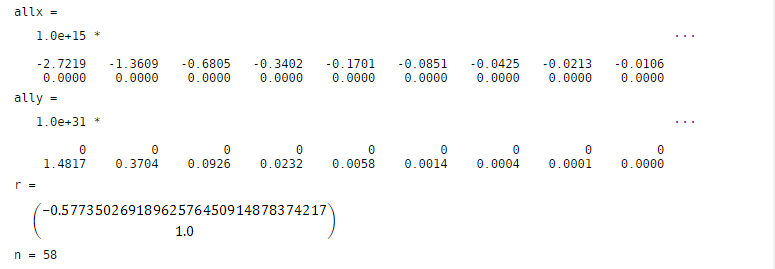
\includegraphics[width=0.9\textwidth]{H3T3D1.png}
                    \caption{n=2时运行结果}
               \end{figure}\\
               
        \end{enumerate}



\end{enumerate}




\end{document}
